\title{Math 239 Fall 2023 Tutorial Review Session}

\date{2023 Nov. 02/03}
\maketitle

% \textbf{Please read:} This week the proposed format is have a bunch of rote questions, and just stand at the board and solve them to try to get through as many questions as possible. For this reason a separate sheet with solutions on it is not important to have -- we should have one sheet with both questions and answers. Recall we should each write about 2 questions each. I think it would be better if we aimed for simpler and shorter questions to be able to show people stuff that they may have forgotten or not understood, such as weight functions or how to get a GF from a recurrence. The only thing I think should be long or ``unusual" are proofs, such as bijections and some graph theory proofs.

% Penny should send us the exam soon, which will help quite a bit on designing questions. I suggest that we design questions in approximately the same ratio as the exam (I will write this later here), but not to cover exactly what is on the exam. I suggest that you do not tell anyone that you have seen the exam either.

% Penny has now sent the exam. There are $8$ multiple choice questions and $6$ long-form questions (with multiple parts for each) The question breakdowns are approximately:
% \begin{itemize}
%     \item Basic counting -- $3$ MC
%     \item Coefficient extraction, recursions, and partial fractions -- $1$ MC and $2$ LF
%     \item Generating function and weight functions -- $3$ MC
%     \item Graph theory -- $1$ MC and $2$ LF
%     \item Bijections -- $1$ LF
%     \item Binary strings -- $1$ LF
% \end{itemize}

% \newpage

\begin{enumerate}
    \question{Bijection Question} Let $n \geq k \geq 2$. Let
    \begin{align*}
        U = \{ \text{$k$-element subsets of $\{ 1, \cdots, n\}$} \}
    \end{align*}
    and
    \begin{align*}
        V = \{ (a,b,A) \}
    \end{align*}
    where
    \begin{align*}
        a &\in \{ 1 , \cdots, n \},\\
        b &\in \{ 0, \cdots, n-a \},\\
        A &\text{ is a $(k-2)$ element subset of $ \{ 1, \cdots, b-1 \}$ }.
    \end{align*}
    (I.e. $V$ is the set of all triples like this). Find a bijection from $U$ to $V$ and use this to show that
    \begin{align*}
        \sum_{i=1}^n \sum_{j=0}^{n-i} \binom{j-1}{k-2} = \binom{n}{k}.
    \end{align*}
    \answer Consider a subset $S$ in $U$. Denote the minimal/maximal element of $S$ as $S_{min} \in \{ 1 , \cdots, n\}$ and $S_{max} \in \{ S_{min} , \cdots, n \}$. Then
    \begin{align*}
        S \subseteq \{ S_{min} , \cdots , S_{max} \}
    \end{align*}
    with $S_{min} , S_{max} \in S$. Write
    \begin{align*}
        T = S \setminus \{ S_{min} , S_{max} \} \subseteq \{ S_{min} + 1 , \cdots , S_{max} - 1 \}.
    \end{align*}
    $T$ has $k-2$ elements. Now write
    \begin{align*}
        a &= S_{min} \in \{ 1 , \cdots, n \},\\
        b &= S_{max} - S_{min} \in \{0 , \cdots, n - S_{min} \} =  \{0 , \cdots, n - a \},\\
        A &= T - S_{min} \subseteq \{ S_{min} - S_{min} + 1 , \cdots , S_{max} - S_{min} - 1 \} = \{ 1 , \cdots , b - 1 \}.
    \end{align*}
    Where our $T - S_{min}$ is element-wise subtraction. Then $(a,b,A)$ is a valid element of $V$. Note that this is clearly bijective, with the inverse being
    \begin{align*}
        (a , b ,A) \mapsto \{ a\}  \cup (A+a) \cup \{ a+b \}
    \end{align*}
    with the $A+a$ being once again element-wise addition.

    Now note that
    \begin{align*}
        |V| &= \sum_{i=1}^n \sum_{j=0}^{n-i} \binom{j-1}{k-2}
    \end{align*}
    where $ \binom{j-1}{k-2}$ counts number of ways to get $A$, $\sum_{j=0}^{n-i} \binom{j-1}{k-2}$ counts the number of ways to get $b$ and $A$, and $\sum_{i=1}^n \sum_{j=0}^{n-i} \binom{j-1}{k-2}$ counts the ways to count elements of $T$. It follows that
    \begin{align*}
        \sum_{i=1}^n \sum_{j=0}^{n-i} \binom{j-1}{k-2} = |V| = |U| = \binom{n}{k}.
    \end{align*}
    
    \question{Coefficient Extraction} Determine the value of the following coefficients. 
    \begin{enumerate}
        \item $[x^{20}]3x^2(1-5x^3)^{-4}$
        \item $[x^{20}]3x^2(1-5x^3)^{-4}(1+x^4)^{-2}$
    \end{enumerate}
    \answer \begin{enumerate}
        \item Apply negative binomial theorem:
        \begin{align*}
            [x^{20}]3x^2(1-5x^3)^{-4} &= 3[x^{18}](1-5x^3)^{-4} \\
            &= 3[x^{18}]\sum_{n\geq 0}\binom{n+4-1}{4-1}(5x^3)^n \\
            &= 3[x^{18}]\sum_{n\geq 0}\binom{n+3}{3}5^nx^{3n} \\
            &= 3 \binom{6+3}{3}5^6\\
            &= 3 \binom{9}{3} \cdot 5^6
        \end{align*}
        \item 
        \begin{align*}
            [x^{20}]3x^2(1-5x^3)^{-4}(1+x^4)^{-2} &= 3[x^{18}](1-5x^3)^{-4}(1+x^4)^{-2} \\
            &=3[x^{18}]\left(\sum_{n\geq 0}\binom{m+4-1}{4-1}(5x^3)^m\right)\left(\sum_{n\geq} \binom{n+2-1}{2-1}(-x^4)^n\right)\\
            &= 3[x^{18}]\left(\sum_{n \geq 0}\binom{m+3}{3}5^mx^{3m}\right)\left(\sum_{n\geq0}(n+1)(-1)^nx^{4n}\right)\\
            &= 3\left(\binom{6+3}{3}5^6(0+1)(-1)^0 + \binom{2+3}{3}5^2(3+1)(-1)^3\right)
            \\
            & \qquad (\text{taking } 3m+4n=18, (m,n) = (6,0), \text{ or } (2,3))
            \\&=3\left(\binom{9}{3}5^6 - \binom{5}{3}5^2\cdot4 \right).
        \end{align*}
    \end{enumerate}
    
    \question{Weight Functions} Are the following functions weight functions?
    \begin{enumerate}
        \item With $S = \mathbb{Z}$, $\omega(n) = n^2$.
        \item With $S = \mathbb{N}$, $\omega(n) = \sqrt{n}$.
        \item With $S = \mathbb{N}$, $w(n) = n \mod k$ for some fixed $k \in \mathbb{N}$.
    \end{enumerate}
    \answer Recall that to be a weight function, a finite number of elements must map to each natural number.
    \begin{enumerate}
        \item Yes, since for each natural number at most $2$ elements map to it.
        \item No, since for example $\sqrt{2} \not\in \mathbb{N}$.
        \item No, since $0 , k , 2k , 3k , \cdots$ all map to $0$, so the pre-image of $0$ is infinite.
    \end{enumerate}

    \newpage
     \question{Binary Substrings} \begin{enumerate}
        \item Give an unambiguous \textit{regular} expression for the set $X$ of all non-empty binary strings that start and end with $1$. Use your regular expression to determine the generating series of $X$ with respect to length.
        \item Give an unambiguous \textit{recursive} expression for the set $Y$ of all non-empty binary strings of at least $3$ blocks, where the string starts and ends with a $0$, and where the first and last blocks have the same size. You solution might make use of part (a) of this question. Use your recursive expression to determine the generating series for $Y$ with respect to length.
    \end{enumerate}
    \answer 

    \begin{enumerate}
        \item An unambiguous regular expression for $X$ is
    \[1 \smile 1 (0 \smile 1)^* 1\]
    The generating series with respect to length is 
    \[\Phi_X(x) = \Phi_1(x) + \Phi_1(x)\Phi_{(0 \smile 1)^*}(x) \Phi_1(x) = x + \frac{x^2}{1-2x} = \frac{x-x^2}{1-2x}.\]
    \item An unambiguous recursive expression for $Y$ is 
    \[Y = 0 (Y \smile X) 0\]
    The generating series with respect to length satisfies 
    \begin{align*}
        \Phi_Y(x) &= \Phi_0(x) (\Phi_Y(x) + \Phi_X(x)) \Phi_0(x) \\
        &= x^2\left(\Phi_Y(x) + \frac{x-x^2}{1-2x}\right) \\
        &= x^2\Phi_Y(x) + \frac{x^3-x^4}{1-2x}
    \end{align*}
    which implies
    \[\Phi_Y(x) = \frac{x^3 - x^4}{(1-2x)(1-x^2)}.\]
    \end{enumerate}

\newpage
    \question{Isomorphism of Graphs} Which of the following graphs are isomorphic? Provide justification. 
    \begin{enumerate}
        \item $G_1$ is the complement of a $6$-cycle. 
        \item $G_2$ is the graph with $V(G)=\{a,b,c,d,e,f\}$ and $E(G)=\{ad, ae, af, bd, be, bf, cd, ce, cf\}$.
        \item $G_3$ is the graph with $V(G)=\{1,2,3,4,5,6\}$ and $E(G)=\{ij | i+j$ is odd $\}$. 
    \end{enumerate}
    \answer Note: I recommend drawing out all three graphs and making the observation that $G_2$ is $K_{3,3}$. Here are $G_1, G_2, G_3$ respectively.

\begin{center}
    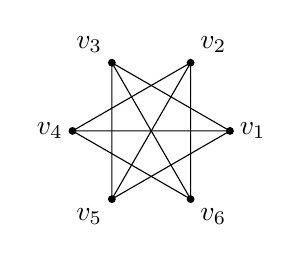
\begin{tikzpicture}
        \coordinate[label = right:$v_1$] (a) at (0:1);
        \coordinate[label = above right:$v_2$] (b) at (60:1);
        \coordinate[label = above left:$v_3$] (c) at (120:1);
        \coordinate[label = left:$v_4$] (d) at (180:1);
        \coordinate[label = below left:$v_5$] (e) at (240:1);
        \coordinate[label = below right:$v_6$] (f) at (300:1);
        
        \node at (a)[circle,fill,inner sep=1pt]{};
        \node at (b)[circle,fill,inner sep=1pt]{};
        \node at (c)[circle,fill,inner sep=1pt]{};
        \node at (d)[circle,fill,inner sep=1pt]{};
        \node at (e)[circle,fill,inner sep=1pt]{};
        \node at (f)[circle,fill,inner sep=1pt]{};

        \draw (a) -- (c) (a) -- (d) (a) -- (e);
        \draw (b) -- (d) (b) -- (e) (b) -- (f);
        \draw (c) -- (e) (c) -- (f);
        \draw (d) -- (f);
    \end{tikzpicture}
    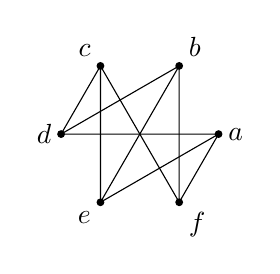
\begin{tikzpicture}
        \coordinate[label = right:$a$] (a) at (0:1);
        \coordinate[label = above right:$b$] (b) at (60:1);
        \coordinate[label = above left:$c$] (c) at (120:1);
        \coordinate[label = left:$d$] (d) at (180:1);
        \coordinate[label = below left:$e$] (e) at (240:1);
        \coordinate[label = below right:$f$] (f) at (300:1);
        
        \node at (a)[circle,fill,inner sep=1pt]{};
        \node at (b)[circle,fill,inner sep=1pt]{};
        \node at (c)[circle,fill,inner sep=1pt]{};
        \node at (d)[circle,fill,inner sep=1pt]{};
        \node at (e)[circle,fill,inner sep=1pt]{};
        \node at (f)[circle,fill,inner sep=1pt]{};

        \draw (a) -- (d) (a) -- (e) (a) -- (f);
        \draw (b) -- (d) (b) -- (e) (b) -- (f);
        \draw (c) -- (d) (c) -- (e) (c) -- (f);
    \end{tikzpicture}
    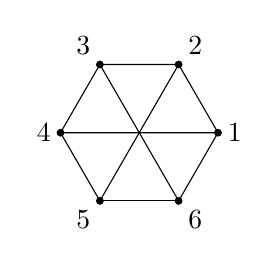
\begin{tikzpicture}
        \coordinate[label = right:$1$] (1) at (0:1);
        \coordinate[label = above right:$2$] (2) at (60:1);
        \coordinate[label = above left:$3$] (3) at (120:1);
        \coordinate[label = left:$4$] (4) at (180:1);
        \coordinate[label = below left:$5$] (5) at (240:1);
        \coordinate[label = below right:$6$] (6) at (300:1);
        
        \node at (1)[circle,fill,inner sep=1pt]{};
        \node at (2)[circle,fill,inner sep=1pt]{};
        \node at (3)[circle,fill,inner sep=1pt]{};
        \node at (4)[circle,fill,inner sep=1pt]{};
        \node at (5)[circle,fill,inner sep=1pt]{};
        \node at (6)[circle,fill,inner sep=1pt]{};

        \draw (1) -- (2) (1) -- (4) (1) -- (6);
        \draw (2) -- (3) (2) -- (5);
        \draw (3) -- (4) (3) -- (6);
        \draw (4) -- (5);
        \draw (5) -- (6);
    \end{tikzpicture}
\end{center}
    
    $G_1$ is not isomorphic to $G_2$ since $G_1$ contains a triangle and $G_2$ is bipartite. Recall that bipartite graphs contain no odd cycles. $G_2$ and $G_3$ are isomorphic. Take for example the function sending $a\rightarrow 1$, $b\rightarrow 3$, $c\rightarrow 5$, $d\rightarrow 2$, $e\rightarrow 4$, and $f\rightarrow 6$. Finally by transitivity of isomorphism $G_1$ and $G)_3$ are not isomorphic. 
    
    \question{Partial Fractions} Use partial fractions to determine and explicit formula for $[x^n]F(x)$ where $F(x)=\frac{1-6x+x^2}{(1-4x)(1-x)^2}$.
    \answer Observe the denominator is already factored so we have $\frac{1-6x+x^2}{(1-4x)(1-x)^2}=\frac{A}{(1-4x)}+\frac{Bx+C}{(1-x)^2}$. Solving for the constants we get $A=\frac{-7}{9}$, $B=\frac{-4}{9}$ and $C=\frac{16}{9}$. This gives $[x^n]F(x)=\frac{-7}{9}4^n+\frac{-4}{9}n(1)^{n}+\frac{16}{9}(1)^n=\frac{-7}{9}4^n+\frac{-4}{9}n+\frac{16}{9}$
    
    \newpage

    % oh no i was going to do this one - alena
    % ah sorry!!!! I misread and asked the wrong person
    % dw :) was just confused lol
    \question{Graph Construction} For $n \ge 2$, let $G_n$ be the graph whose vertices are permutations of $\{1, \dots, n\}$, where we have an edge between two permutations if we can obtain one from the other by swapping two elements. 
    \begin{enumerate}
        \item Draw $G_3$ and label its vertices. 
        \item Show that this graph is regular, find the degree.
        
    \end{enumerate}
    \answer \begin{enumerate}
        \item Using the notation $\sigma = (\sigma_1 , \sigma_2 , \sigma_3)$:

\begin{center}
    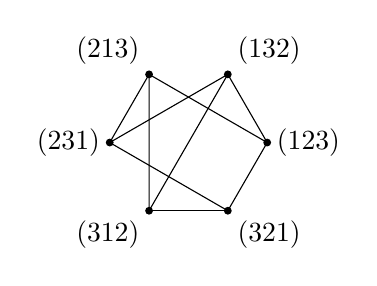
\begin{tikzpicture}
        \coordinate[label = right:$(123)$] (123) at (0:1);
        \coordinate[label = above right:$(132)$] (132) at (60:1);
        \coordinate[label = above left:$(213)$] (213) at (120:1);
        \coordinate[label = left:$(231)$] (231) at (180:1);
        \coordinate[label = below left:$(312)$] (312) at (240:1);
        \coordinate[label = below right:$(321)$] (321) at (300:1);
        
        \node at (123)[circle,fill,inner sep=1pt]{};
        \node at (132)[circle,fill,inner sep=1pt]{};
        \node at (213)[circle,fill,inner sep=1pt]{};
        \node at (231)[circle,fill,inner sep=1pt]{};
        \node at (312)[circle,fill,inner sep=1pt]{};
        \node at (321)[circle,fill,inner sep=1pt]{};

        \draw (123) -- (132) (123) -- (213) (123) -- (321);
        \draw (132) -- (231) (132) -- (312);
        \draw (213) -- (231) (213) -- (312);
        \draw (231) -- (321);
        \draw (312) -- (321);
    \end{tikzpicture}
\end{center}


        \item Degree should be $n \choose 2$ because a vertex $v$ will be adjacent to permutations that are obtained from $v$ by two elements swapping places, so we pick $2$ elements to swap out of $n$.
        
    \end{enumerate}
   
    \newpage
    
    \question{Compositions} How many integer compositions of $n$ consist of either 5 or 6 parts, where each part is even?
    \answer For a partition with only even parts, we want $A = \{2, 4, 6, \dots\}$ with weight function $w(a) = a$, which gives us generating series $\Phi_A(x) = x^2 + x^4 + x^6 + \dots = \frac{x^2}{1-x^2}$.
    
    The set we are counting is $A^5 \cup A^6$, which is a disjoint union, so we can apply the sum lemma to get $\Phi_S(x) = \Phi_{A^5}(x) + \Phi_{A^6}(x)$.

    By the product lemma, we have 
    \begin{center}
        $\Phi_{A^5}(x) = (\Phi_{A}(x))^5 = (\frac{x^2}{1-x^2})^5 =  \frac{x^{10}}{(1-x^2)^5}$

        $\Phi_{A^6}(x) = (\Phi_{A}(x))^6 = (\frac{x^2}{1-x^2})^6 =  \frac{x^{12}}{(1-x^2)^6}$
    \end{center}

    So \begin{center}
        $\Phi_S(x) = \frac{x^{10}}{(1-x^2)^5} + \frac{x^{12}}{(1-x^2)^6} = \frac{x^{10} - x^{12} + x^{12}}{(1-x^2)^6} = \frac{x^{10}}{(1-x^2)^6}$
    \end{center}

    The number of integer compositions of $n$ consisting of 5 or 6 even parts is 

    \begin{center}
        $[x^n]\Phi_S(x) = [x^n]\frac{x^{10}}{(1-x^2)^6} = [x^{n-10}](1-x^2)^{-6} =  \begin{cases} 
          0 & n\ \mathrm{is}\ \mathrm{odd} \\
          {\frac{n-10}{2} + 5 \choose 5} & n\ \mathrm{is}\ \mathrm{even} 
       \end{cases}$
    \end{center}

    
    
\end{enumerate}


